\chapter{\IfLanguageName{dutch}{Opzetten lokale testomgeving}{Introduction}}
\label{ch:testlokaal}

In dit hoofdstuk wordt besproken hoe de lokale testomgevingen zijn opgezet. Er zijn 3 lokale testomgevingen. De eerste is één die cloud-init gebruikt, de tweede gebruikt Ansible en de derde gebruikt cloud-init en Anisble. Voor het opzetten wordt er VirtualBox en Vagrant gebruikt.

\section{Cloud-init}
De eerste testomgeving die wordt besproken is de omgeving met cloud-init. Deze wordt opgezet met behulp van: \autocite{cloudVagrant}. Er wordt hiervoor in 2 stappen gewerkt. Eerst wordt een ISO met de cloud-init configuraties aangemaakt met behulp van de setup van \autocite{cloudVagrant}. Daarna wordt deze ISO toegevoegd aan de testomgeving.

\subsection{Maken van ISO met cloud-init configuraties}
Voor het aanmaken van de ISO er een Linux omgeving nodig. Allereest wordt er een omgeving opgezet om de ISO's in te maken. Deze wordt ook opgezet met Vagrant en VirtualBox. De box \textit{ubuntu/xenial64} wordt gebruikt (dit is dezelfde als degene die later in de testomgeving wordt gebruikt). Met het commando \textit{vagrant up} wordt de server aangemaakt. De vagrantfile ziet er zo uit:
\begin{lstlisting}
Vagrant.configure(''2'') do |config|
config.vm.box =''ubuntu/xenial64''
end
\end{lstlisting}

Via het commando \textit{vagrant ssh} is er toegang tot de server. Zodra deze toegang tot de machine er is , wordt de package \textit{genisoimage} geïnstalleerd. Dit gebeurt via het commando \textit{sudo apt-get install genisoimage}. 

Nadat die package geïnstalleerd is, wordt een user-data bestand aangemaakt. In dit bestand komt de cloudconfig data. Hierna wordt een tweede bestand aangemaakt, het meta-data bestand. In dit bestand komt nog extra minimale configuratie. De local-hostname en instance-id moeten hierin worden gezet.

Als deze bestanden zijn aangemaakt wordt een Makefile gecreëerd. Via dit bestand wordt de iso aangmaakt. De Makefile ziet er als volgt uit:
\begin{lstlisting}
nocloud.iso: meta-data user-data
mkisofs \
-joliet -rock \
-volid "cidata" \
-output nocloud.iso meta-data user-data
\end{lstlisting}

Ten laatste wordt het \textit{make} package geïnstalleerd. Via het commando \textit{make} wordt het iso bestand aangemaakt.

\subsection{Opzetten van testomgeving met cloud-init configuraties}
Een tweede omgeving wordt aangemaakt (de effectieve testomeving) opnieuw doormiddel van Vagrant en VirtualBox. Net zoals in het vorige gedeelte wordt ook hier de box \textit{ubuntu/xenial64} gebruikt.

In het vorige gedeelte is het iso bestand aangemaakt met de cloud-init configuraties. Allereerst moet dit iso bestand worden gekopieerd naar de map van de omgeving. In de vagrantfile die wordt gebruikt moet worden doorverwezen naar deze iso. Dit wordt gedaan met deze configuraties in de vagrantfile.
\begin{lstlisting}
IMAGE_PATH = File.join(File.dirname(__FILE__), "no-cloud.iso")

Vagrant.configure(2) do |config|

config.vm.box = "ubuntu/xenial64"

config.ssh.password = nil	
config.vm.synced_folder ".", "/vagrant", disabled: true

config.vm.provider :virtualbox do |vb|
vb.customize [
"storageattach", :id,
"--storagectl", "SCSI",
"--port", "1",
"--type", "dvddrive",
"--medium", IMAGE_PATH
]
vb.linked_clone = true
end
end
\end{lstlisting}
Als hierna \textit{vagrant up} wordt gedaan, wordt de server aangemaakt met de configuraties van cloud-init.

\section{Ansible}
De tweede lokale testomgeving die wordt opgezet is die met Ansible. Deze is minder complex om op te zetten dan degene met cloud-init. Dat er maar één machine nodig is. Deze wordt opgezet met behulp van \autocite{ansibleVagrant}. Ook deze omgeving gebruikt Vagrant en VirtualBox. Als box wordt ook opnieuw dezelfde gebruikt als de vorige keren. 

Het opzetten van de testomgeving gebeurt in 4 stappen. 

Allereerst wordt een vagrantfile aangemaakt. In dit vagrantfile wordt verwezen naar het playbook, de inventory en de map waar deze zich bevinden. Via dit vagrantfile is het ook mogelijk om ansible uit te voeren met vagrant via een Windows systeem. Het vagrantfile ziet er als volgt uit.:
\begin{lstlisting}
# -*- mode: ruby -*-
# vi: set ft=ruby :

Vagrant.configure("2") do |config|
config.vm.box = "ubuntu/xenial64"

config.vm.provider "virtualbox" do |vb|
vb.memory = "1024"
end

config.vbguest.auto_update = false
config.vbguest.no_install = false
config.vbguest.no_remote = true

config.vm.hostname = "ansible-teslocal"

config.vm.provision "ansible_local" do |ansible|
ansible.provisioning_path = "/vagrant/provisioning"
ansible.inventory_path = "inventory"
ansible.playbook = "playbook.yml"
ansible.limit = "all"
end

end
\end{lstlisting}

Hierna wordt de map \textit{provisioning} aangemaakt in de de map van de omgeving. In die map worden 3 bestanden aangemaakt. Allereerst een \textit{ansible.cfg} bestand. Hierin worden configuraties gezet zodat Vagrant en Ansible niet ''panikeren'' over ssh sleutels.
\begin{lstlisting}
[defaults]
host_key_checking = no
[ssh_connection]
ssh_args = -o ControlMaster=auto -o ControlPersist=60s -o UserKnownHostsFile=/dev/null -o IdentitiesOnly=yes
\end{lstlisting}
Het tweede bestand is een inventory bestand. Hierin wordt gezet welke host aanwezig is en welke connectie deze heeft.
\begin{lstlisting}
ansible-test-local ansible_connection=local
\end{lstlisting}

Het derde bestand dat wordt aangemaakt is het effectieve playbook.

Het laatste dat wordt gedaan is het installeren van de vagrant-plugin \textit{vbguest}. Dit wordt gedaan met het commando \textit{vagrant plugin install vagrant-vbguest}.

Als nu \textit{vagrant up} wordt gedaan, wordt de server opgestart met de configuraties van Ansible.

\section{Cloud-init \& Ansible }
De derde omgeving die wordt opgezet is één met Ansible en cloud-init. Zoals wordt beschreven zijn er voor Puppet en Chef aparte modules om configuraties uit te voeren. Voor Ansible is dit echter niet het geval. Dus moet een creatieve oplossing gezocht worden. Voor de combinatie van Ansible en cloud-init wordt met de \textit{write\_files} module in cloud-init gewerkt. 

\subsection{Ansible playbook koppelen aan cloud-init}
Een server wordt lokaal aangemaakt met de manier van cloud-init. Er wordt wel een bestand toegevoegd met module \textit{write\_files}. Dit bestand is het playbook van de server. De content van het bestand moet wel worden geëncodeerd via de Base64 standaard. Dit wordt gedaan via de tool: https://codebeautify.org/base64-encode. In de tekst wordt de te encoderen tekst gezet. Daarna wordt in het andere tekstvak de geëncodeerde versie gegeven. Met deze tool wordt het playbook geëncodeerd.
\begin{figure}[!htb]
	\center{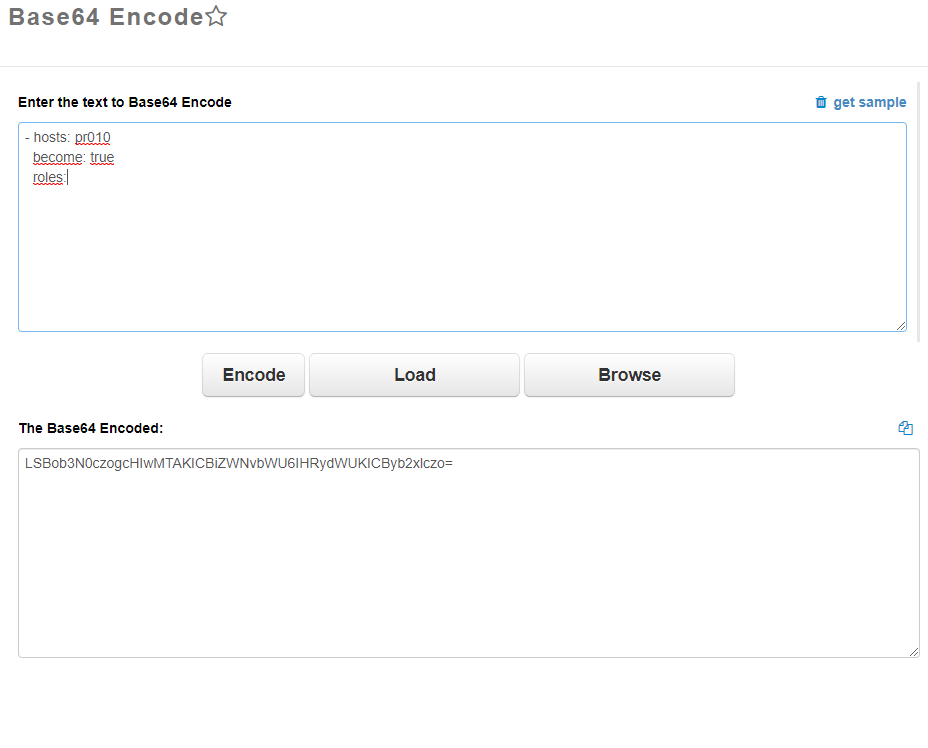
\includegraphics[width=0.9\textwidth]{img/base64.png}}
	\caption{Tool voor encoding.}
	\label{fig:base64}
\end{figure}

\newpage
\subsection{Uitvoeren playbook}
Als het playbook in de \textit{write\_files} module staat, moeten nog 2 dingen gebeuren. 

Allereest moet de package \textit{ansible} worden geïnstalleerd via cloud-init. Dit werd gedaan door \textit{ansible} toe te voegen aan de module \textit{packages}. 

Ook moet het playbook worden aangeroepen om te draaien. Dit gebeurt door bij de module \textit{runcmd} het commando \textit{ansible-playbook -i, <aangemaakt playbook>} te zetten.

Via deze omgeving kunnen cloud-init en Ansible configuraties worden gedaan.



